\documentclass[11pt,a4paper]{article}

% --- Kodowanie i język ---
\usepackage[utf8]{inputenc}
\usepackage[T1]{fontenc}
\usepackage{lmodern}
\usepackage[polish]{babel}

% --- Grafika, tabele, układ ---
\usepackage{graphicx}
\usepackage{booktabs}
\usepackage{float}
\usepackage{caption}
\usepackage[margin=2.5cm]{geometry}
\usepackage{microtype}
\usepackage{enumitem}

% --- Kod źródłowy ---
\usepackage{xcolor}
\usepackage{listings}
\definecolor{codekw}{RGB}{0,90,160}
\definecolor{codecomment}{RGB}{110,110,110}
\definecolor{codestr}{RGB}{160,60,30}
\definecolor{codebg}{RGB}{248,248,248}
\lstset{
  language=Python,
  basicstyle=\ttfamily\small,
  keywordstyle=\color{codekw}\bfseries,
  commentstyle=\color{codecomment}\itshape,
  stringstyle=\color{codestr},
  backgroundcolor=\color{codebg},
  frame=single,
  rulecolor=\color{gray!40},
  breaklines=true,
  showstringspaces=false,
  numbers=left,
  numberstyle=\tiny\color{gray},
  captionpos=b,
  literate=%
    {ą}{{\k a}}1 {ć}{{\'c}}1 {ę}{{\k e}}1 {ł}{{\l}}1 {ń}{{\'n}}1
    {ó}{{\'o}}1 {ś}{{\'s}}1 {ż}{{\.z}}1 {ź}{{\'z}}1
    {Ą}{{\k A}}1 {Ć}{{\'C}}1 {Ę}{{\k E}}1 {Ł}{{\L}}1 {Ń}{{\'N}}1
    {Ó}{{\'O}}1 {Ś}{{\'S}}1 {Ż}{{\.Z}}1 {Ź}{{\'Z}}1
}

% --- Hyperref na końcu ---
\usepackage[hidelinks]{hyperref}

\title{\textbf{Klasyfikacja fake-news: sieć neuronowa TF-IDF $\rightarrow$ MLP}\\[0.3em]
\large Dokumentacja techniczna --- Sztuczne Sieci Neuronowe}
\author{Aleksander Oleszkiewicz}
\date{\today}

\begin{document}

\maketitle
\begin{abstract}
\noindent
Dokument opisuje pierwszą sieć neuronową budowaną od zera w ramach projektu pracy
dyplomowej --- binarny klasyfikator fałszywych wiadomości oparty na reprezentacji
\textbf{TF-IDF} i wielowarstwowej sieci gęstej (\textbf{MLP}) w PyTorchu. Omawiamy
analizę i czyszczenie danych (w tym eliminację wycieku informacji), architekturę i
proces uczenia modelu, metryki ewaluacji wraz z diagnozą bias--variance, kluczowe
komponenty kodu oraz przykładowe predykcje. Model osiąga F1 i ROC-AUC na poziomie
$\sim$0{,}99 na zbiorze testowym, stanowiąc zweryfikowany fundament pod docelowy
model BiLSTM + Attention.
\end{abstract}

\tableofcontents
\vspace{1em}

\section{Wstęp}

\subsection{Problem}

Automatyczne wykrywanie fałszywych wiadomości (\emph{fake-news}) to zadanie
klasyfikacji binarnej: na podstawie treści artykułu prasowego model rozstrzyga,
czy pochodzi on z wiarygodnego źródła (\emph{Real}), czy jest dezinformacją
(\emph{Fake}). Trudność problemu nie leży w samym dopasowaniu klasyfikatora ---
jak pokażemy, klasy są w tym zbiorze silnie rozróżnialne leksykalnie --- lecz w
\textbf{rzetelnym przygotowaniu danych}: zbiór zawiera liczne sygnały wycieku
informacji (ang. \emph{data leakage}), które pozwalają uzyskać niemal perfekcyjne
metryki bez uczenia się treści. Większość pracy projektowej dotyczy więc
identyfikacji i usunięcia tych sygnałów, tak by model uczył się stylu i tematyki, a
nie artefaktów technicznych.

\subsection{Cel}

Celem tego etapu jest zbudowanie \textbf{pierwszej sieci neuronowej od zera}
(bez wag pretrenowanych, bez fine-tuningu i feature-tuningu --- zgodnie z wymogiem
przedmiotu SSN) oraz zweryfikowanie kompletnej pętli treningowej w PyTorchu
(propagacja wsteczna, optymalizator Adam, early stopping, regularyzacja, obsługa
GPU). Stanowi to fundament pod model docelowy pracy dyplomowej:
\textbf{BiLSTM + Attention} z osadzeniami GloVe~300d.

\subsection{Zbiór danych}

Wykorzystujemy publiczny zbiór \emph{Fake and Real News Dataset} (Kaggle,
\texttt{clmentbisaillon/fake-and-real-news-dataset}) --- dwa pliki CSV
(\texttt{True.csv}, \texttt{Fake.csv}) z artykułami prasowymi w języku angielskim.
W całym projekcie obowiązuje konwencja etykiet:
\[
  \texttt{1 = Real}, \qquad \texttt{0 = Fake}.
\]
Model operuje wyłącznie na kolumnie \texttt{text}; kolumny \texttt{title},
\texttt{subject} i \texttt{date} są odrzucane jako źródła wycieku informacji
(uzasadnienie w sekcji~\ref{sec:dane}).

\section{Analiza i przygotowanie danych}
\label{sec:dane}

\subsection{Statystyki zbioru}

Surowy zbiór liczy \textbf{44\,898} artykułów o niemal zrównoważonych klasach
($\sim$52\% Fake / 48\% Real). Eksploracyjna analiza danych
(\texttt{notebooks/explore/01\_eda.ipynb}) ujawniła dwa istotne problemy jakości:

\begin{itemize}[noitemsep]
  \item \textbf{Duplikaty}: ok. 13{,}9\% artykułów to dokładne duplikaty tekstu,
        skupione niemal wyłącznie w klasie Fake (ok. 25{,}7\% artykułów Fake vs
        1{,}1\% Real). Brak konfliktów etykiet między klasami --- deduplikacja jest bezpieczna.
  \item \textbf{Puste / bardzo krótkie teksty}: ok. 1{,}4\% rekordów (głównie wpisy
        Fake zawierające jedynie odnośnik do YouTube).
\end{itemize}

Po pełnym potoku czyszczenia i deduplikacji pozostaje \textbf{38\,470} artykułów
(Fake: 17\,281 = 44{,}9\%, Real: 21\,189 = 55{,}1\%). Rozkład długości tekstu jest
silnie prawoskośny; 95.~percentyl to ok. \textbf{900 słów} --- wartość przyjęta jako
kandydat na \texttt{max\_seq\_len} w docelowym modelu sekwencyjnym.

\subsection{Wyciek informacji (data leakage)}

Analiza w \texttt{notebooks/explore/02\_leakage.ipynb} wykorzystała informację
wzajemną (Mutual Information, MI) oraz test $\chi^2$ do oceny siły poszczególnych
markerów jako predyktorów klasy. Najsilniejsze sygnały (Tabela~\ref{tab:leakage})
to artefakty redakcyjno-techniczne, a nie cechy treści: nagłówek agencyjny
``\texttt{(Reuters)}'' pozwala niemal jednoznacznie wskazać klasę Real.

\begin{table}[H]
  \centering
  \caption{Najsilniejsze markery wycieku wg informacji wzajemnej (MI).}
  \label{tab:leakage}
  \begin{tabular}{lcl}
    \toprule
    \textbf{Marker} & \textbf{MI [nat]} & \textbf{Dominująca klasa} \\
    \midrule
    słowo ,,reuters''            & 0{,}650 & Real \\
    dateline ,,MIASTO (Reuters) -- '' & 0{,}456 & Real \\
    ,,featured image''           & 0{,}136 & Fake \\
    \texttt{@handle} (media społ.)& 0{,}076 & Fake \\
    ,,getty (images)''           & 0{,}061 & Fake \\
    prefiks clickbait (VIDEO/WATCH) & 0{,}018 & Fake \\
    \bottomrule
  \end{tabular}
\end{table}

Wniosek z analizy: kolumna \texttt{subject} rozdziela klasy w 100\% (każda kategoria
należy w całości do jednej klasy), a \texttt{title} oraz \texttt{date} również niosą
silny wyciek (Fake: 83\% tytułów ALL-CAPS; daty Fake w niestandardowym formacie).
Wszystkie trzy kolumny są więc odrzucane --- model korzysta wyłącznie z \texttt{text}.

\subsection{Czyszczenie tekstu}

Funkcja \texttt{clean\_text} (\texttt{src/data/cleaning.py}) stosuje uporządkowaną
kaskadę wyrażeń regularnych --- każdy wzorzec ma uzasadnienie w analizie MI powyżej.
Kolejność operacji jest istotna (np.\ usunięcie ,,via @handle'' przed samym
\texttt{@handle}, rozdzielenie ,,2017World'' przed sprowadzeniem do małych liter):

\begin{enumerate}[noitemsep]
  \item markery agencyjne Reuters (dateline, ,,(Reuters)'', słowo ,,reuters'');
  \item adresy URL (\texttt{http(s)}, \texttt{www}, \texttt{pic.twitter.com}, \texttt{tmsnrt.rs});
  \item uchwyty mediów społecznościowych (\texttt{@handle}, ,,via @\dots'');
  \item prefiksy clickbait (\texttt{VIDEO:}, \texttt{WATCH:}, \texttt{BREAKING:});
  \item szablony podpisów zdjęć (,,featured image via getty'', ,,photo by\dots'');
  \item artefakty HTML (znaczniki, encje, bloki \texttt{<script>});
  \item sygnatury serwisów (,,21st Century Wire'');
  \item normalizacja: białe znaki, usunięcie pojedynczych znaków, małe litery.
\end{enumerate}

Po czyszczeniu stosowany jest filtr \texttt{filter\_short\_articles} z progiem
\textbf{\texttt{min\_words = 10}} (usuwa głównie wpisy-zaślepki Fake). Walidacja w
\texttt{04\_post\_cleaning.ipynb} potwierdza, że kluczowe markery (dateline, URL,
\texttt{@handle}, getty) spadają do 0\% wystąpień, a pokrycie słownika GloVe pozostaje
wysokie (OOV $\le$ 0{,}2\%).

\subsection{Podział na zbiory}

Funkcja \texttt{make\_splits} (\texttt{src/data/splits.py}) dzieli dane
\textbf{stratyfikowanie} po etykiecie na zbiory train/val/test w proporcji
60/20/20 (dwukrotne wywołanie \texttt{train\_test\_split}), ze stałym ziarnem
\texttt{RANDOM\_STATE} dla powtarzalności (Tabela~\ref{tab:splits}). Balans klas
($\sim$44{,}9\% Fake / 55{,}1\% Real) jest zachowany we wszystkich trzech zbiorach.

\begin{table}[H]
  \centering
  \caption{Podział stratyfikowany na zbiory.}
  \label{tab:splits}
  \begin{tabular}{lcc}
    \toprule
    \textbf{Zbiór} & \textbf{Liczba artykułów} & \textbf{Udział} \\
    \midrule
    train & 23\,082 & 60\% \\
    val   & 7\,694  & 20\% \\
    test  & 7\,694  & 20\% \\
    \midrule
    razem & 38\,470 & 100\% \\
    \bottomrule
  \end{tabular}
\end{table}

\section{Architektura modelu}
\label{sec:arch}

\subsection{Reprezentacja tekstu: TF-IDF}

Tekst jest zamieniany na wektor cech metodą \textbf{TF-IDF} (\emph{Term
Frequency--Inverse Document Frequency}). Jest to nieparametryczna inżynieria cech ---
\emph{nie} model pretrenowany --- więc model neuronowy w całości uczy się od zera.
Wektoryzator (\texttt{make\_tfidf\_vectorizer}, \texttt{src/model/baseline.py}) jest
\textbf{współdzielony} z baselinem (regresją logistyczną), co zapewnia uczciwe
porównanie obu klasyfikatorów. Jest dopasowywany \textbf{wyłącznie na zbiorze
treningowym}, a tym samym słownikiem transformowane są val i test (brak wycieku
ze zbiorów ewaluacyjnych). Parametry zebrano w Tabeli~\ref{tab:tfidf}.

\begin{table}[H]
  \centering
  \caption{Konfiguracja wektoryzatora TF-IDF.}
  \label{tab:tfidf}
  \begin{tabular}{ll}
    \toprule
    \textbf{Parametr} & \textbf{Wartość} \\
    \midrule
    \texttt{max\_features} & 50\,000 (rozmiar słownika) \\
    \texttt{ngram\_range}  & (1, 2) --- unigramy i bigramy \\
    \texttt{min\_df}       & 5 (minimalna częstość dokumentowa) \\
    \texttt{sublinear\_tf} & \texttt{True} ($1 + \log(\mathrm{tf})$) \\
    \texttt{strip\_accents}& \texttt{"unicode"} \\
    \bottomrule
  \end{tabular}
\end{table}

\subsection{Sieć gęsta (MLP)}

Klasyfikatorem jest wielowarstwowa sieć gęsta (\texttt{MLPClassifier},
\texttt{src/model/mlp.py}) o architekturze:
\[
  \underbrace{\text{Linear}(50\,000, 256)}_{\text{warstwa ukryta}}
  \;\rightarrow\; \text{ReLU}
  \;\rightarrow\; \text{Dropout}(0{,}3)
  \;\rightarrow\; \underbrace{\text{Linear}(256, 1)}_{\text{wyjście (logit)}}.
\]
Wyjściem jest pojedynczy \emph{logit} (bez sigmoidy), co pozwala użyć numerycznie
stabilnej funkcji straty \texttt{BCEWithLogitsLoss}. Sieć liczy
\textbf{12\,800\,513} parametrów --- zdecydowana większość przypada na pierwszą
warstwę ($50\,000 \times 256$), bo wymiar wejścia równy jest rozmiarowi słownika.

\subsection{Proces uczenia}

Funkcja \texttt{train\_mlp} realizuje pełną pętlę treningową z \textbf{early
stopping} monitorującym F1 na zbiorze walidacyjnym i przywracającym wagi z najlepszej
epoki (Tabela~\ref{tab:train}). W praktyce trening zatrzymał się po \textbf{11
epokach} (z dozwolonych 20).

\begin{table}[H]
  \centering
  \caption{Hiperparametry uczenia.}
  \label{tab:train}
  \begin{tabular}{ll}
    \toprule
    \textbf{Parametr} & \textbf{Wartość} \\
    \midrule
    optymalizator        & Adam \\
    learning rate        & $1\times10^{-3}$ \\
    funkcja straty       & \texttt{BCEWithLogitsLoss} \\
    rozmiar batcha        & 256 \\
    maks. epok           & 20 \\
    early stopping       & na F1 walidacji, \texttt{patience = 3} \\
    dropout              & 0{,}3 \\
    weight decay (L2)    & 0 (domyślnie; badany w sekcji~\ref{sec:eval}) \\
    próg decyzyjny       & 0{,}5 \\
    ziarno losowe        & \texttt{RANDOM\_STATE} (powtarzalność) \\
    \bottomrule
  \end{tabular}
\end{table}

\paragraph{Uzasadnienie wyborów.}
Funkcja \texttt{BCEWithLogitsLoss} łączy sigmoidę z entropią krzyżową w sposób
numerycznie stabilny i jest naturalna dla klasyfikacji binarnej. Adam zapewnia szybką
zbieżność bez ręcznego strojenia harmonogramu uczenia. Early stopping na F1 (a nie na
stracie) jest spójny z metryką raportowaną i chroni przed przeuczeniem przy
praktycznie zerowym koszcie. Dropout 0{,}3 to standardowa, umiarkowana regularyzacja
warstwy ukrytej.

\section{Ewaluacja}
\label{sec:eval}

\subsection{Metryki na walidacji i teście}

Model oceniamy pięcioma metrykami (Tabela~\ref{tab:metrics}). Wszystkie utrzymują się
na poziomie $\sim$0{,}99, co dla tego zbioru oznacza praktyczny sufit jakości.

\begin{table}[H]
  \centering
  \caption{Metryki MLP na zbiorze walidacyjnym i testowym.}
  \label{tab:metrics}
  \begin{tabular}{lcc}
    \toprule
    \textbf{Metryka} & \textbf{Walidacja} & \textbf{Test} \\
    \midrule
    accuracy  & 0{,}9908 & 0{,}9864 \\
    precision & 0{,}9899 & 0{,}9838 \\
    recall    & 0{,}9934 & 0{,}9915 \\
    F1        & 0{,}9916 & 0{,}9877 \\
    ROC-AUC   & 0{,}9992 & 0{,}9987 \\
    \bottomrule
  \end{tabular}
\end{table}

\begin{figure}[H]
  \centering
  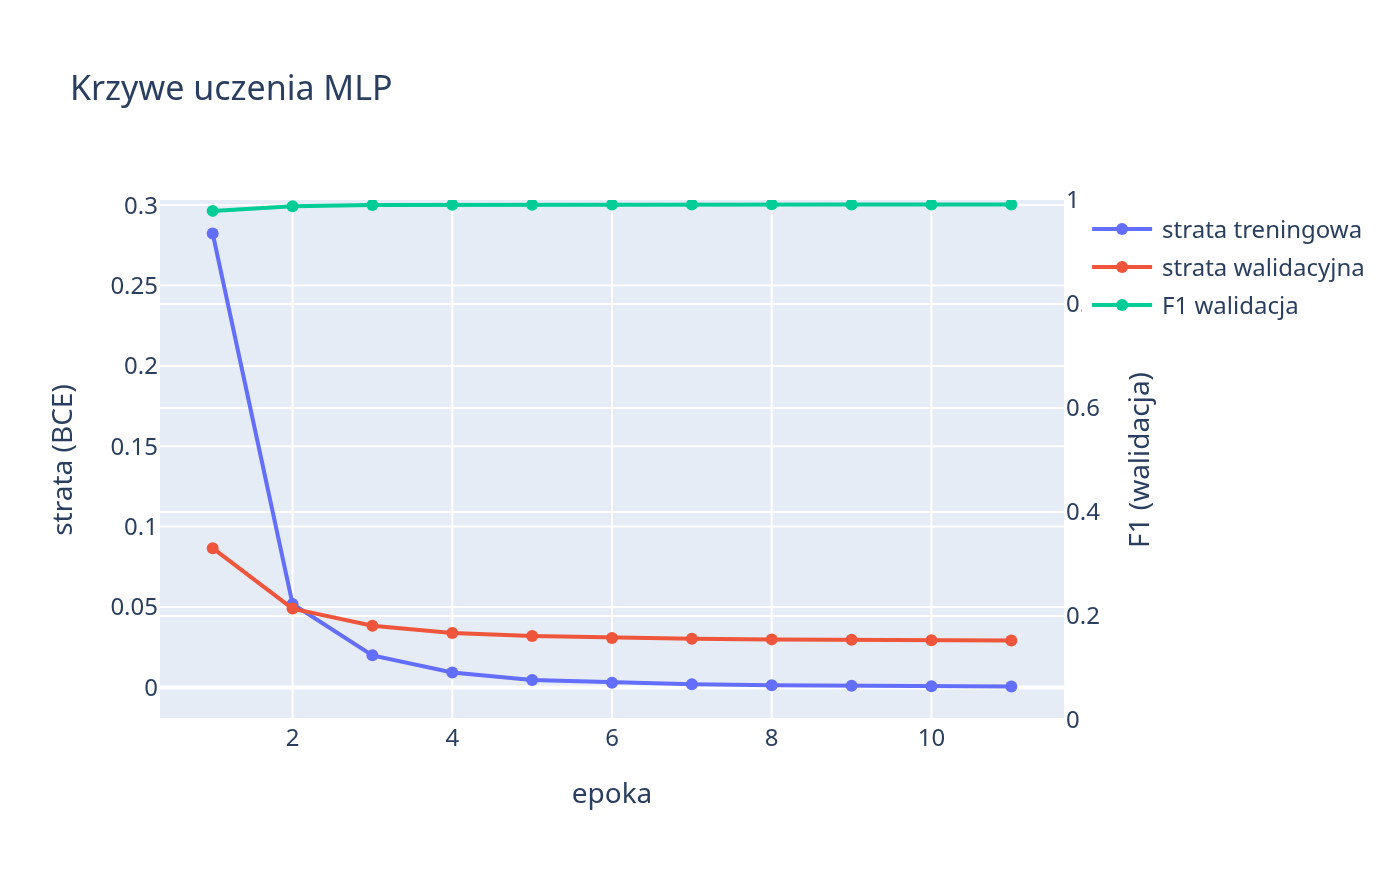
\includegraphics[width=0.78\textwidth]{figures/mlp_krzywe_uczenia.png}
  \caption{Krzywe uczenia MLP: strata treningowa/walidacyjna (oś lewa) oraz F1
  walidacji (oś prawa). Sieć zbiega w pierwszych epokach; early stopping przerywa
  trening, gdy F1 przestaje rosnąć.}
\end{figure}

\begin{figure}[H]
  \centering
  \begin{minipage}{0.48\textwidth}
    \centering
    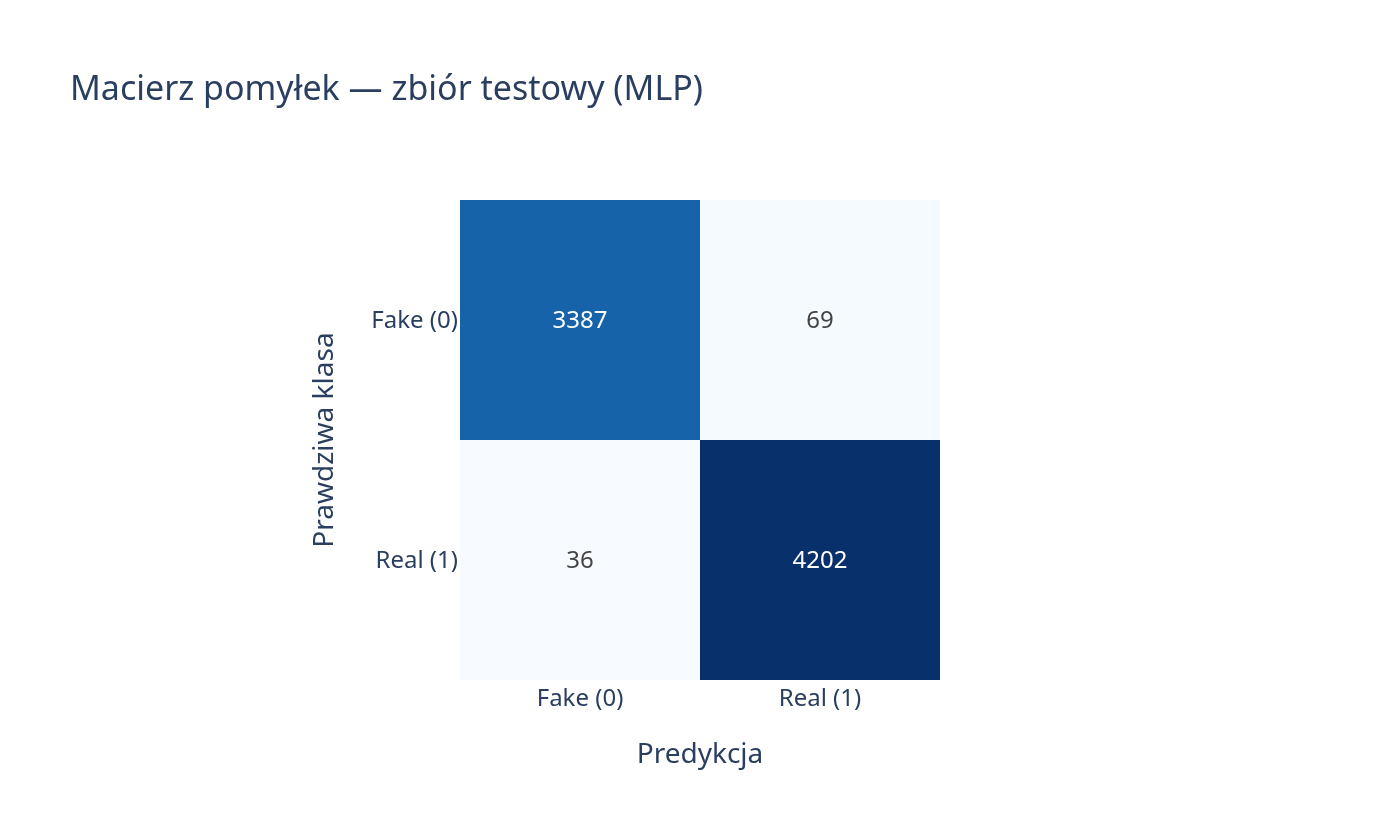
\includegraphics[width=\textwidth]{figures/mlp_macierz_pomylek.png}
  \end{minipage}\hfill
  \begin{minipage}{0.48\textwidth}
    \centering
    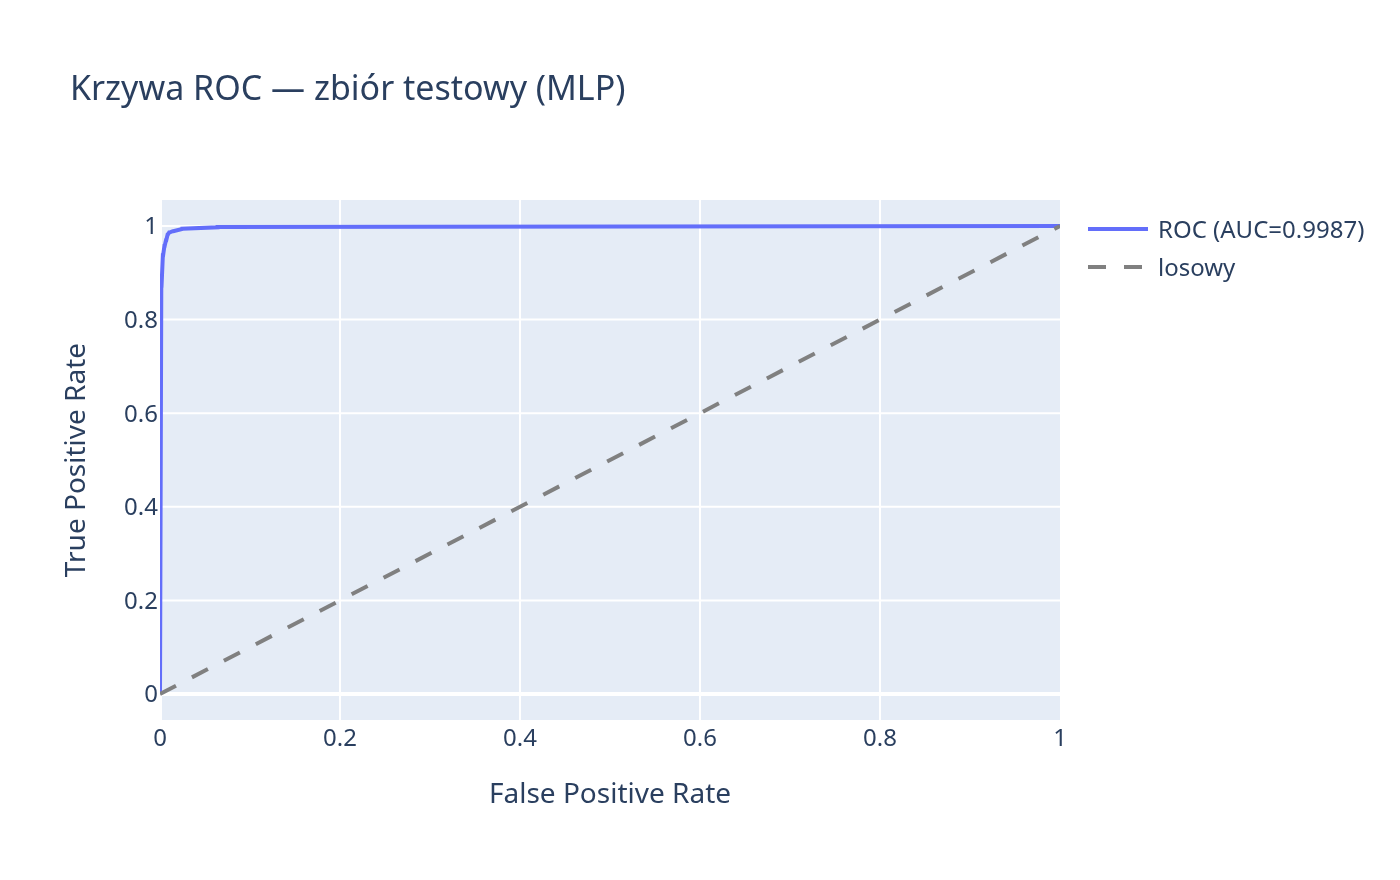
\includegraphics[width=\textwidth]{figures/mlp_roc.png}
  \end{minipage}
  \caption{Macierz pomyłek (po lewej) i krzywa ROC (po prawej) na zbiorze testowym.
  Błędy są nieliczne i rozłożone na obie klasy.}
\end{figure}

\subsection{Porównanie z baselinem (LogReg vs MLP)}

Ponieważ oba modele korzystają z \emph{identycznej} reprezentacji TF-IDF, różnica
wyników izoluje wpływ samej architektury klasyfikatora (Tabela~\ref{tab:compare}).

\begin{table}[H]
  \centering
  \caption{Porównanie na zbiorze testowym.}
  \label{tab:compare}
  \begin{tabular}{lcc}
    \toprule
    \textbf{Metryka} & \textbf{LogReg (baseline)} & \textbf{MLP (od zera)} \\
    \midrule
    accuracy  & 0{,}9795 & \textbf{0{,}9864} \\
    precision & 0{,}9751 & \textbf{0{,}9838} \\
    recall    & 0{,}9880 & \textbf{0{,}9915} \\
    F1        & 0{,}9815 & \textbf{0{,}9877} \\
    ROC-AUC   & 0{,}9970 & \textbf{0{,}9987} \\
    \bottomrule
  \end{tabular}
\end{table}

MLP przewyższa baseline o ok.\ 0{,}6~pp F1 --- różnica marginalna. Na tym leksykalnie
łatwym zbiorze klasy są niemal liniowo separowalne w przestrzeni TF-IDF, więc
nieliniowość sieci nie daje istotnej przewagi. Wartością tego etapu jest nie wzrost
metryk, lecz zweryfikowana pętla treningowa w PyTorchu.

\subsection{Diagnoza bias--variance}

Krzywa uczenia (trening na rosnących podzbiorach 10--100\% przy ustalonym
wektoryzatorze) izoluje wpływ liczby przykładów. Obie krzywe F1 leżą wysoko i blisko
siebie (Tabela~\ref{tab:lc}, Rys.~\ref{fig:lc}): F1 treningowe $\approx$1{,}0
(\textbf{niski bias}), a luka train--val maleje do $\sim$0{,}8~pp wraz z liczbą
przykładów (\textbf{niska wariancja}). Krzywa walidacyjna szybko wchodzi na plateau ---
dokładanie danych nie podniesie metryki.

\begin{table}[H]
  \centering
  \caption{Krzywa uczenia --- F1 vs liczba przykładów treningowych.}
  \label{tab:lc}
  \begin{tabular}{cccc}
    \toprule
    \textbf{$n_{\text{train}}$} & \textbf{F1 train} & \textbf{F1 val} & \textbf{luka} \\
    \midrule
    2\,308  & 1{,}0000 & 0{,}9710 & 0{,}0290 \\
    5\,770  & 1{,}0000 & 0{,}9812 & 0{,}0188 \\
    11\,540 & 1{,}0000 & 0{,}9871 & 0{,}0129 \\
    17\,312 & 1{,}0000 & 0{,}9899 & 0{,}0101 \\
    23\,082 & 1{,}0000 & 0{,}9916 & 0{,}0084 \\
    \bottomrule
  \end{tabular}
\end{table}

\begin{figure}[H]
  \centering
  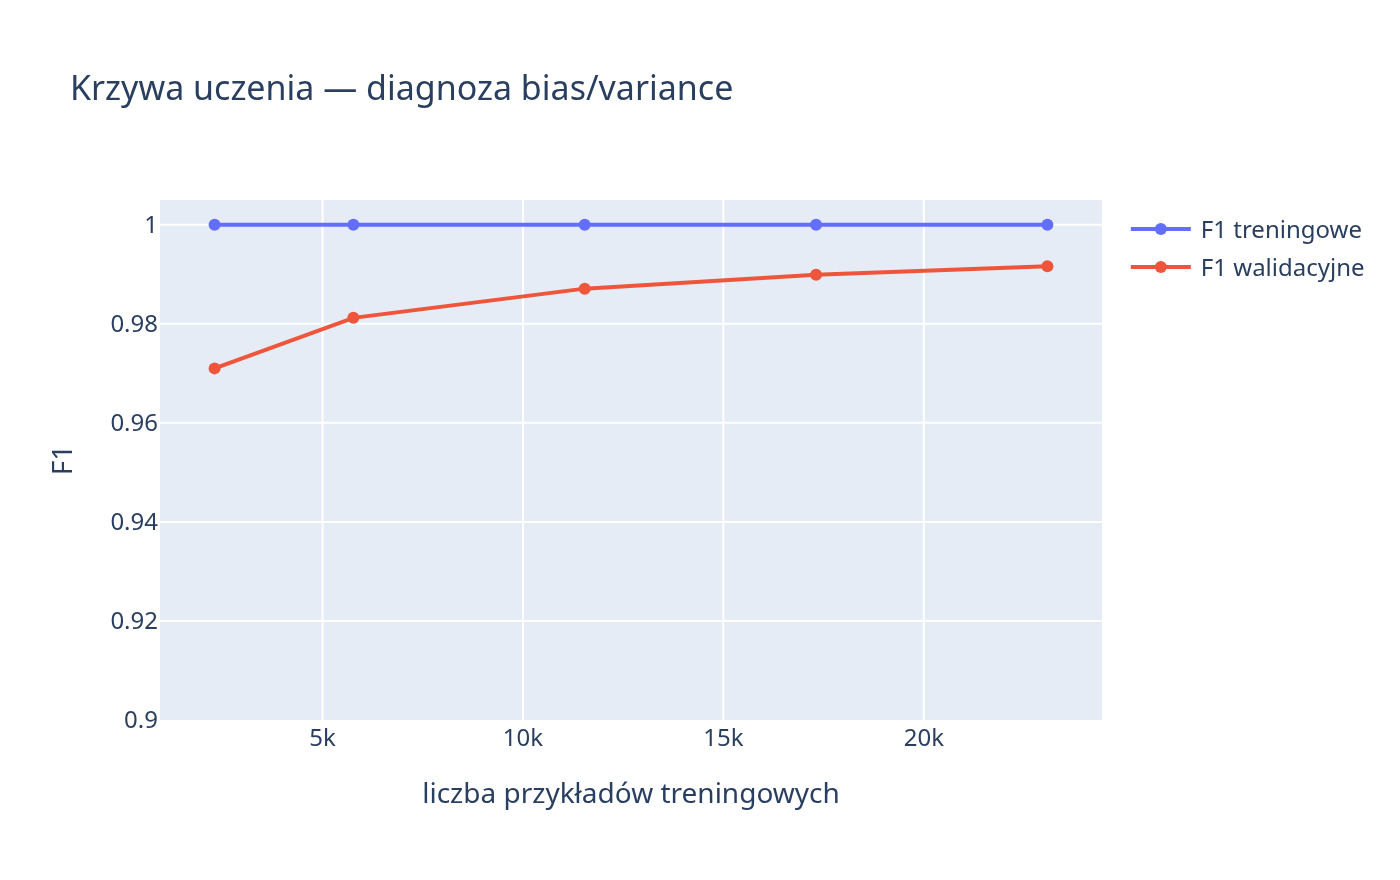
\includegraphics[width=0.72\textwidth]{figures/mlp_learning_curve.png}
  \caption{Krzywa uczenia. Obie krzywe wysoko i blisko siebie --- reżim
  niskiego biasu i niskiej wariancji przy suficie metryk zbioru.}
  \label{fig:lc}
\end{figure}

\subsection{Techniki regularyzacji}

Choć przeuczenie jest tu łagodne, model umożliwia jego kontrolę trzema technikami:
early stopping (zawsze aktywny), dropout i weight decay (L2). Tabela~\ref{tab:reg}
pokazuje wpływ na lukę train--val (miarę wariancji).

\begin{table}[H]
  \centering
  \caption{Wpływ regularyzacji na lukę train--val F1.}
  \label{tab:reg}
  \begin{tabular}{lccc}
    \toprule
    \textbf{Konfiguracja} & \textbf{F1 train} & \textbf{F1 val} & \textbf{luka} \\
    \midrule
    brak (dropout=0, wd=0) & 1{,}0000 & 0{,}9913 & 0{,}0087 \\
    dropout=0{,}3          & 1{,}0000 & 0{,}9916 & 0{,}0084 \\
    L2 (wd=$10^{-4}$)      & 0{,}9987 & 0{,}9939 & 0{,}0048 \\
    dropout=0{,}3 + L2     & 0{,}9987 & 0{,}9933 & 0{,}0054 \\
    \bottomrule
  \end{tabular}
\end{table}

Dropout i weight decay zmniejszają lukę (obniżają F1 treningowe, podtrzymując
walidacyjne), lecz F1 walidacyjne ledwie drga --- przy tak łatwym zbiorze
regularyzacja głównie kosmetyzuje lukę, a nie poprawia uogólnienia. Potwierdza to
diagnozę z krzywej uczenia.

\subsection{Interpretowalność cech}

Współczynniki regresji logistycznej (baseline) dają tanią, globalną wyjaśnialność
(Rys.~\ref{fig:cechy}). Stronę Real ciągną zwroty agencyjno-sprawozdawcze
(\texttt{said}, \texttt{on wednesday}, \texttt{president donald}), stronę Fake ---
zwroty potoczne/clickbaitowe (\texttt{via}, \texttt{read more}, \texttt{you},
\texttt{watch}, \texttt{video}). Co istotne, \emph{żaden} z usuniętych markerów
wycieku nie pojawia się na liście --- model uczy się stylu i tematu, a nie stempla
redakcyjnego.

\begin{figure}[H]
  \centering
  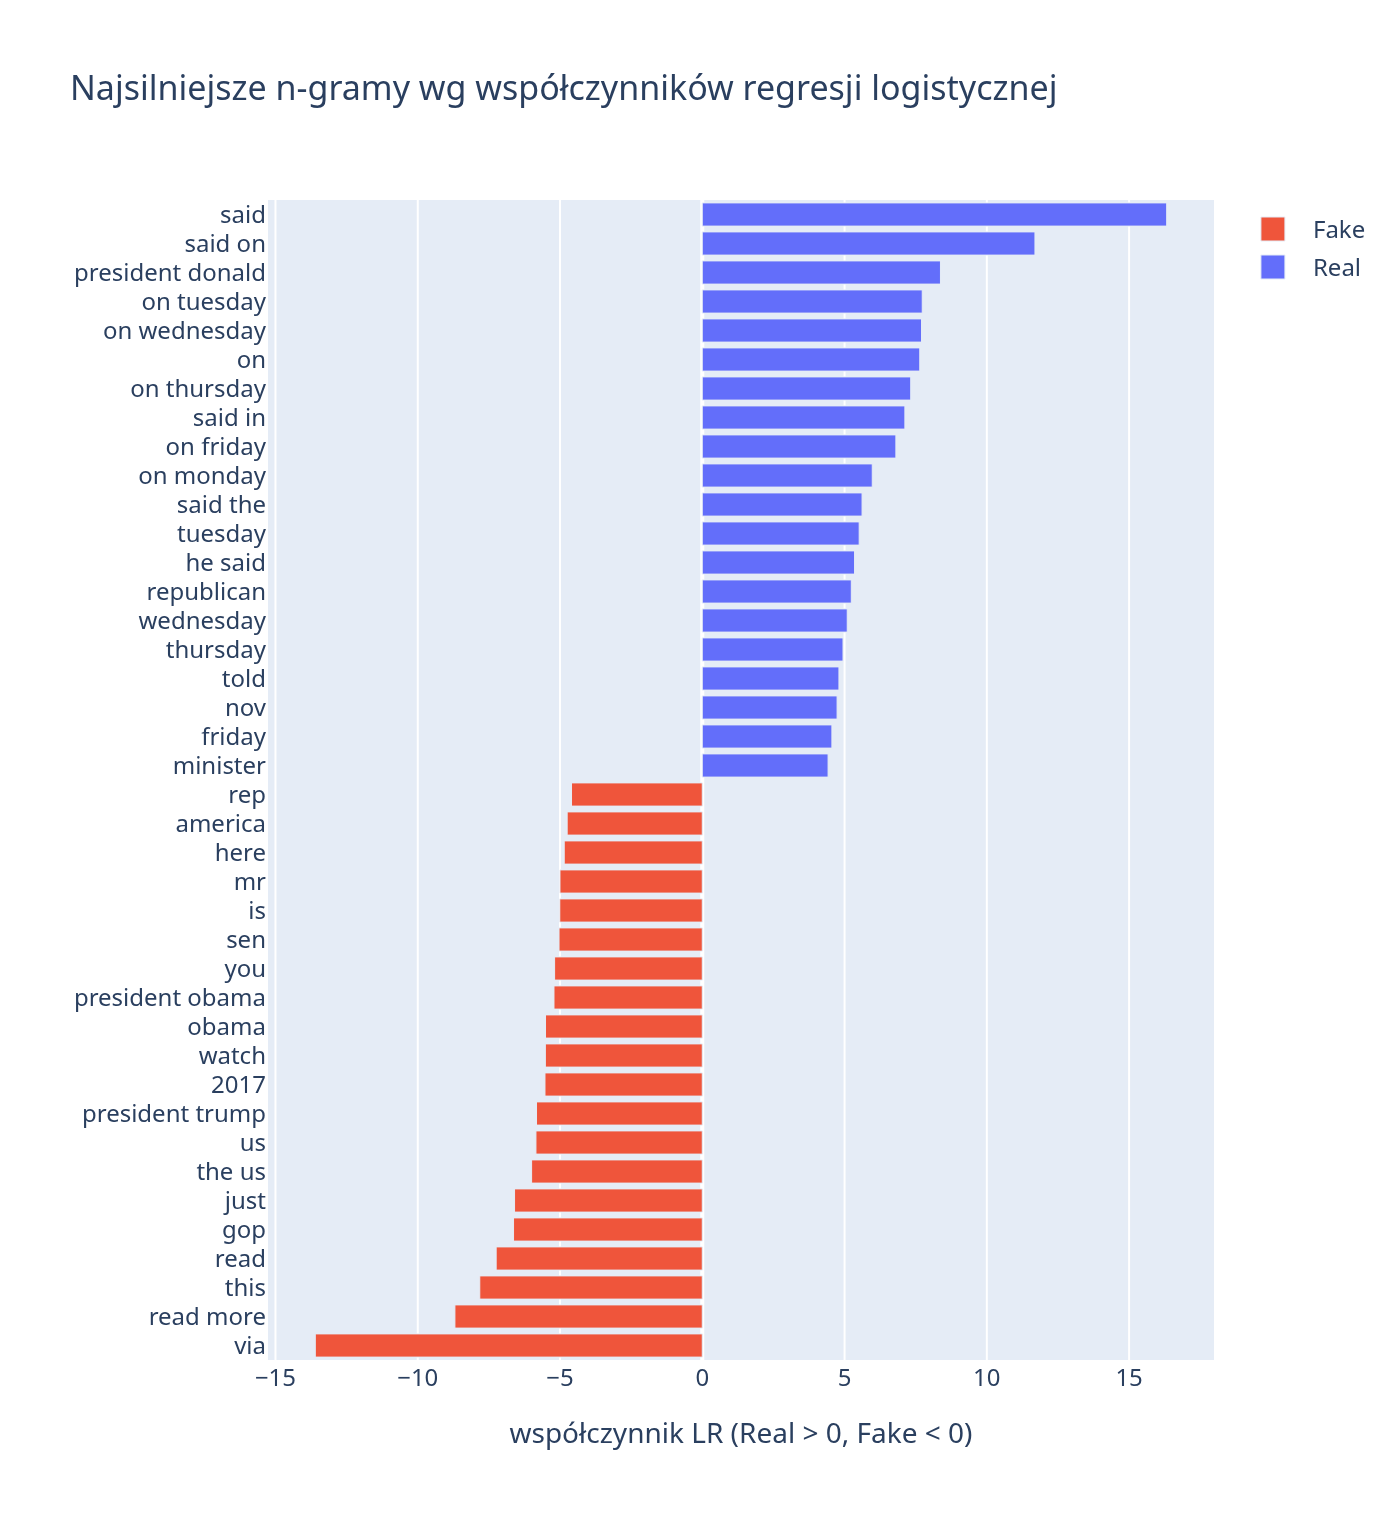
\includegraphics[width=0.85\textwidth]{figures/logreg_cechy.png}
  \caption{Najsilniejsze n-gramy wg współczynników regresji logistycznej
  (Real $> 0$, Fake $< 0$).}
  \label{fig:cechy}
\end{figure}

\section{Przykładowe predykcje}
\label{sec:predykcje}

Aby pokazać działanie sieci na konkretnych artykułach, dla każdego tekstu ze zbioru
testowego obliczono prawdopodobieństwo $P(\text{Real})$ i porównano z progiem
0{,}5. Tabela~\ref{tab:pred} zestawia dwa pewne trafienia każdej klasy oraz oba typy
błędów: \emph{false positive} (Fake uznane za Real) i \emph{false negative} (Real
uznane za Fake).

\begin{table}[H]
  \centering
  \caption{Przykładowe predykcje MLP na zbiorze testowym (próg 0{,}5).}
  \label{tab:pred}
  \small
  \begin{tabular}{p{6.6cm}cccc}
    \toprule
    \textbf{Fragment tekstu} & \textbf{Prawdziwa} & \textbf{P(Real)} & \textbf{Predykcja} & \\
    \midrule
    \multicolumn{5}{l}{\emph{Pewne trafienia}}\\
    \addlinespace[2pt]
    ,,germany foreign minister said on saturday that\dots'' & Real & 1{,}0000 & Real & \checkmark \\
    ,,china called for ceasefire in myanmar rakhine\dots''  & Real & 1{,}0000 & Real & \checkmark \\
    ,,patrick henningsen the longer this soap opera\dots''  & Fake & 0{,}0000 & Fake & \checkmark \\
    ,,patrick henningsen despite repeated failures\dots''   & Fake & 0{,}0000 & Fake & \checkmark \\
    \addlinespace[3pt]
    \multicolumn{5}{l}{\emph{Błędy: false positive (Fake $\to$ Real)}}\\
    \addlinespace[2pt]
    ,,the washington post nearly third of territory\dots''  & Fake & 0{,}9998 & Real & $\times$ \\
    ,,leading from behind hasn worked out so well\dots''    & Fake & 0{,}9997 & Real & $\times$ \\
    \addlinespace[3pt]
    \multicolumn{5}{l}{\emph{Błędy: false negative (Real $\to$ Fake)}}\\
    \addlinespace[2pt]
    ,,- below are the highlights from oct. 25 excl\dots''   & Real & 0{,}0015 & Fake & $\times$ \\
    ,,the emmy awards show was peppered with politic\dots'' & Real & 0{,}0059 & Fake & $\times$ \\
    \bottomrule
  \end{tabular}
\end{table}

\paragraph{Kalibracja i omówienie błędów.}
Prawdopodobieństwa $P(\text{Real})$ są \textbf{nasycone na krańcach}
($\approx$0 dla Fake, $\approx$1 dla Real), również w przypadku pomyłek: artykuły
Fake błędnie zaklasyfikowane jako Real otrzymują $P(\text{Real})\approx0{,}9998$.
Model jest zatem \textbf{silny w rankingu} (ROC-AUC 0{,}9987), lecz \textbf{przepewny
i słabo skalibrowany}: myli się rzadko, ale gdy się myli, robi to z wysoką pewnością,
zamiast sygnalizować niepewność wartościami w pobliżu progu 0{,}5. Same błędy dotyczą
tekstów stylistycznie ,,pogranicznych'', co \emph{sugeruje} (lecz nie dowodzi)
związek z cechami z sekcji~\ref{sec:eval}:

\begin{itemize}[noitemsep]
  \item \textbf{False positive} (Fake $\to$ Real): teksty otwierające się
        frazą agencyjno-prasową (np.\ ,,the washington post\dots''), stylistycznie
        zbliżone do źródeł wiarygodnych;
  \item \textbf{False negative} (Real $\to$ Fake): teksty nietypowe dla klasy Real,
        sformatowane jako lista (,,- below are the highlights\dots'') lub o tematyce
        rozrywkowej (gala Emmy) zamiast politycznej/agencyjnej.
\end{itemize}

Błędy są więc rzadkie i koncentrują się na artykułach ,,pogranicznych'' stylistycznie,
co jest spójne z nielicznymi pomyłkami w macierzy pomyłek (Rys.~\ref{sec:eval}).
Wysoka pewność tych pomyłek pozostaje jednak sygnałem ograniczonej kalibracji modelu.

\section{Kluczowe komponenty kodu}
\label{sec:kod}

Cała logika modelu jest wydzielona do \texttt{src/model/mlp.py} i pokryta testami
jednostkowymi (\texttt{tests/model/}). Poniżej omówiono najistotniejsze fragmenty.

\subsection{\texttt{TfidfDataset}: leniwa densyfikacja}

Macierz TF-IDF jest rzadka (50\,000 kolumn, lecz nieliczne niezerowe wartości w
wierszu). Gęste zmaterializowanie całego korpusu naraz byłoby kosztowne pamięciowo,
dlatego \texttt{TfidfDataset} przechowuje dane jako macierz rzadką i densyfikuje
\emph{pojedynczy wiersz dopiero przy pobraniu} przez \texttt{DataLoader}.

\begin{lstlisting}[caption={Leniwa densyfikacja wiersza w \texttt{TfidfDataset}.}]
def __getitem__(self, index: int) -> tuple[torch.Tensor, torch.Tensor]:
    row = self.features[index].toarray().ravel().astype(np.float32, copy=False)
    return torch.from_numpy(row), self.labels[index]
\end{lstlisting}

\subsection{\texttt{MLPClassifier}: sieć zwracająca logity}

Sieć budowana jest jako stos bloków \texttt{Linear $\to$ ReLU $\to$ Dropout},
zakończony pojedynczą warstwą liniową. \texttt{forward} zwraca surowe \emph{logity}
(bez sigmoidy), co pozwala użyć numerycznie stabilnej \texttt{BCEWithLogitsLoss}
w treningu, a \texttt{torch.sigmoid} dopiero przy wnioskowaniu.

\begin{lstlisting}[caption={Konstrukcja warstw \texttt{MLPClassifier}.}]
layers: list[nn.Module] = []
in_features = input_dim
for width in hidden_dims:
    layers.append(nn.Linear(in_features, width))
    layers.append(nn.ReLU())
    layers.append(nn.Dropout(dropout))
    in_features = width
layers.append(nn.Linear(in_features, 1))
self.net = nn.Sequential(*layers)
\end{lstlisting}

\subsection{\texttt{train\_mlp}: pętla treningowa z early stopping}

Pętla naprzemiennie trenuje (\texttt{\_train\_one\_epoch}) i waliduje
(\texttt{\_validate}, zwraca stratę i F1). Po każdej epoce, jeśli F1 walidacji
poprawił się, zapisywany jest stan wag; w przeciwnym razie zliczane są epoki bez
poprawy, a po przekroczeniu \texttt{patience} trening zostaje przerwany. Na końcu
przywracane są najlepsze wagi.

\begin{lstlisting}[caption={Rdzeń early stopping w \texttt{train\_mlp}.}]
optimizer = torch.optim.Adam(model.parameters(), lr=lr, weight_decay=weight_decay)
criterion = nn.BCEWithLogitsLoss()
...
for _ in range(epochs):
    train_loss = _train_one_epoch(model, train_loader, optimizer, criterion, dev)
    val_loss, val_f1 = _validate(model, val_loader, criterion, dev)
    ...
    if val_f1 > best_val_f1:
        best_val_f1 = val_f1
        best_state = {n: t.detach().cpu().clone()
                      for n, t in model.state_dict().items()}
        epochs_without_improvement = 0
    else:
        epochs_without_improvement += 1
        if epochs_without_improvement >= patience:
            break
if best_state:
    model.load_state_dict(best_state)
\end{lstlisting}

\subsection{\texttt{predict\_proba} i \texttt{evaluate\_mlp}}

\texttt{predict\_proba} przepuszcza dane przez sieć w trybie ewaluacji i zwraca
$P(\text{Real})$ jako tablicę \texttt{numpy} (logit $\to$ \texttt{sigmoid}).
\texttt{evaluate\_mlp} owija to w obliczenie metryk i zwraca \emph{dokładnie taki
sam słownik} (\texttt{accuracy}, \texttt{precision}, \texttt{recall}, \texttt{f1},
\texttt{roc\_auc}, \texttt{confusion\_matrix}) co \texttt{baseline.evaluate}, dzięki
czemu porównanie obu modeli jest bezpośrednie.

\subsection{Reprodukowalność i urządzenie}

\texttt{set\_seed} ustawia ziarno dla NumPy oraz PyTorcha (CPU i CUDA/ROCm), a
\texttt{resolve\_device} automatycznie wybiera GPU, gdy jest dostępne (na maszynie
deweloperskiej działa build ROCm, dla którego \texttt{torch.cuda.is\_available()}
zwraca \texttt{True}). Oba modele korzystają z tego samego wektoryzatora
(\texttt{baseline.make\_tfidf\_vectorizer}), co gwarantuje identyczną reprezentację
tekstu i uczciwe porównanie architektur.

\section{Wnioski i dalsze kroki}

\subsection{Podsumowanie}

\begin{itemize}[noitemsep]
  \item \textbf{TF-IDF $\rightarrow$ MLP} to sieć neuronowa zbudowana w całości
        od zera (bez fine-/feature-tuningu), zgodna z wymogiem przedmiotu SSN.
        Działa na tych samych splitach, konwencji etykiet i wektoryzatorze co
        baseline, a cała logika jest reużywalna w \texttt{src/model/mlp.py}.
  \item Model osiąga F1 i ROC-AUC na poziomie $\sim$0{,}99 na zbiorze testowym,
        co jest wynikiem porównywalnym z baselinem (regresją logistyczną). Na tym leksykalnie
        łatwym zbiorze sieć nie zyskuje istotnej przewagi nad modelem liniowym.
  \item Diagnoza \textbf{bias-variance} (krzywa uczenia + sweep regularyzacji)
        wskazuje reżim \textbf{niskiego biasu i niskiej wariancji} przy suficie
        metryk zbioru: powiększanie modelu ani zbioru przyniosłoby co najwyżej
        marginalną poprawę, a regularyzacja jedynie domyka niewielką lukę train-val.
  \item Przykładowe predykcje ujawniają, że model jest \textbf{przepewny}:
        prawdopodobieństwa są nasycone na krańcach również przy pomyłkach (słaba
        kalibracja mimo wysokiego ROC-AUC). Nieliczne błędy dotyczą tekstów
        stylistycznie ,,pogranicznych'' (agencyjny styl w artykułach Fake, format
        listy lub tematyka rozrywkowa w artykułach Real).
\end{itemize}

\subsection{Ograniczenia}

Najważniejszym ograniczeniem jest \textbf{sufit metryczny} zbioru: po usunięciu
wycieku klasy nadal różnią się na tyle silnie leksykalnie, że proste reprezentacje
(TF-IDF) wystarczają do niemal perfekcyjnej klasyfikacji. Utrudnia to wykazanie
przewagi bardziej złożonych architektur na tym konkretnym zbiorze. Model
worka słów (TF-IDF) z założenia ignoruje też \textbf{kolejność i kontekst} słów.

\subsection{Dalsze kroki}

Projekt dostarcza zweryfikowaną pętlę treningową PyTorcha (Adam,
\texttt{BCEWithLogitsLoss}, early stopping, dropout, weight decay, obsługa GPU) oraz
kompletny, reużywalny kod modelu w \texttt{src/model/mlp.py}. Naturalnym kierunkiem
dalszego rozwoju, poza zakresem niniejszego projektu, jest architektura
\textbf{BiLSTM + Attention} z osadzeniami \textbf{GloVe~300d}: w odróżnieniu od worka
słów modelowałaby kontekst sekwencyjny, a mechanizm atencji umożliwiłby
\textbf{wyjaśnialność na poziomie pojedynczego artykułu} (wizualizację wag atencji).


\begin{thebibliography}{9}
\bibitem{dataset} C.~Bisaillon, \emph{Fake and Real News Dataset}, Kaggle.
  \url{https://www.kaggle.com/datasets/clmentbisaillon/fake-and-real-news-dataset}.
\bibitem{glove} J.~Pennington, R.~Socher, C.~D.~Manning,
  \emph{GloVe: Global Vectors for Word Representation}, EMNLP 2014.
\bibitem{pytorch} A.~Paszke i in.,
  \emph{PyTorch: An Imperative Style, High-Performance Deep Learning Library},
  NeurIPS 2019.
\bibitem{sklearn} F.~Pedregosa i in.,
  \emph{Scikit-learn: Machine Learning in Python}, JMLR 12, 2011.
\end{thebibliography}

\end{document}
